\chapter{Polarisation des Lichts}
Als Polarisation des Lichts bezeichnet man die (wohldefinierte) Richtung des elektrischen Feldvektors $\vec{E}$ im Bezug auf die Ausbreitungsrichtung $\vec{k}$ der Welle. Wie derartiges Licht erzeugt und nachgewiesen wird, sowie seine Eigenschaften, sollen in diesem Versuch erschlossen werden. 

Hierzu soll zunächst die mathematische Beschreibung von elektromagnetischen Wellen wiedergegeben werden. Dies geschieht durch die Maxwellgleichungen und die daraus abgeleiteten elektromagnetischen Wellengleichungen:
\begin{align}
	\label{eq:4}\divg{E}&=0\\
	\label{eq:6}\divg{B}&=0\\
	\rot{B}&=\epsilon_0\epsilon_r\pdiff{\vec{E}}{t}\\
	\label{eq:5}\rot{E}&=-\mu_0\pdiff{\vec{B}}{t}\\
	\Lap\vec{E}-\mu_0&\epsilon_0\epsilon_r\pddiff{\vec{E}}{t}=0\\
	\Lap\vec{B}-\mu_0&\epsilon_0\epsilon_r\pddiff{\vec{B}}{t}=0
\end{align}
Hieraus lässt sich mit der Lichtgeschwindigkeit $\sol=\frac{1}{\sqrt{\mu_0\epsilon_0}}$ leicht die wohlbekannte Lösung in Form einer ebenen Welle verifizieren.

Bei der Polarisation von Licht unterscheidet man hauptsächlich drei Fälle: linear, zirkular und elliptisch polarisiertes Licht. Vom ersten Fall spricht man, wenn die Schwingebene ortsfest ist, sich also bei der Projektion der Schwingung auf eine zur Ausbreitungsrichtung senkrechte Ebene das Bild einer geraden Linie ergibt. Man erhält diese Form der Polarisation bei der Überlagerung gleichamplitudiger, linear polarisierter Wellen mit Phasendifferenz $\Delta\varphi=k\cdot\pi,~ k\in\IZ$. Eine weitere Möglichkeit ist die Überlagerung gleich intensiver zirkular polarisierter Wellen. Die Richtung der Polarisation hängt dann von der Phasendifferenz der ursprünglichen Wellen ab.

Der Spezialfall der zirkular polarisierten Welle entsteht dann, wenn amplitudengleiche Wellen mit einer Phasendifferenz $\Delta\varphi=(k+\frac{1}{2})\pi,~k\in\IZ$ überlagert werden, bzw. bei der Überlagerung zirkular polarisierter Wellen, wobei die eine eine verschwindend geringe Amplitude besitzt. In jedem anderen Fall ergibt sich der allgemeine Fall einer elliptisch polarisierten Welle.

Im Folgenden sollen außerdem Methoden zur Erzeugung polarisierten Lichts diskutiert werden. Hierzu ist zunächst ein weiterer mathematischer Zusammenhang vonnöten, der die Intensität von Licht beschreibt, das einen idealen Polfilter durchläuft: Das Gesetz von Malus
\begin{equation}
	I(\theta)=I_0\cos^2\theta
\end{equation}
Im Fall unpolarisierten Lichtes muss noch über alle möglichen Winkel integriert werden:
\begin{equation}
	\avg{I}=\frac{1}{2\pi}\int_{0}^{2\pi}I_0\cos^2\theta\d\theta=\frac{1}{2}I_0
\end{equation}

Eine besonders in diesem Versuch, sowie zur Erzeugung sogenannter $\lambda/4-$ und $\lambda/2-$Plättchen wichtige Möglichkeit zur Lichtpolarisation ist die Doppelbrechung in Kristallen mit optischen Achsen. Dies passiert, wenn ein Kristall optisch anisotrop ist und mehrere ausgezeichnete Richtungen besitzt, entlang derer Licht gleicher Wellenlänge, aber unterschiedlicher Polarisation unterschiedlich stark gebrochen werden. So können für die sich aufspaltenden Lichtstrahlen bestimmte Gangunterschiede über die Dicke der Kristallplatte festgelegt werden. 

Ein ähnliches Prinzip liegt der optischen Aktivität organischer Moleküle zugrunde. Mittels bereits bekannter Werte für den spezifischen Drehwinkel eines bestimmten Stoffes kann so recht einfach seine Konzentration in einer Lösung bestimmt werden.
\section{Vorbereitung}
\begin{enumerate}
	\item Unter welchen Voraussetzungen sind die Maxwellgleichungen \eqref{eq:4}-\eqref{eq:5} gültig?
		\subitem Die Gleichungen gelten für ungeladene, stromfreie lineare Materialien mit skalaren Größen $\mu_r,\epsilon_r$. Im Fall anisotroper Materialien werden diese durch entsprechende Tensoren $\ten{\mu}_r,\ten{\epsilon}_r$ ersetzt.
	\item Unter welchen Bedingungen sind ebene Wellen Lösungen der Maxwellgleichungen?
		\subitem Die ebenen Wellen müssen die Dispersionsrelation $\omega=\sol k$, sowie die Transversalitätsbedingung $\skp{E}{k}=0$ bzw. $\skp{B}{k}=0$ erfüllen.
	\item Zeigen Sie, dass elektromagnetische Wellen Transversalwellen sind.
		\subitem Betrachte elektromagnetische Wellen der Form:
		\begin{align*}
			\vec{E}(\vec{r},t)&=\vec{E}_0\e{\imath(kz-\omega t)}\\
			\vec{B}(\vec{r},t)&=\vec{B}_0\e{\imath(kz-\omega t)}
		\end{align*}
		Im Zweifelsfall kann das zugrundeliegende Koordinatensystem immer so gelegt werden, dass $\vec{k}\cdot\uvec{z}=0$ gilt. Durch Einsetzen in die Maxwellgleichungen \eqref{eq:4} und \eqref{eq:6} ergibt sich folgende Bedingung:
		\begin{align*}
			\divg{E}&=E_{0,z}\e{\imath(kz-\omega t)}=0&&\Rightarrow E_{0,z}=0\\
			\divg{B}&=B_{0,z}\e{\imath(kz-\omega t)}=0&&\Rightarrow B_{0,z}=0
		\end{align*}
		Die Wellen stehen also senkrecht auf ihrer Ausbreitungsrichtung und sind somit transversal.
	\item Warum ist das natürliche Licht unpolarisiert?
		\subitem Natürliches Licht, wie z.B. Sonnenlicht ist als thermische Strahlung aus vielen Einzelwellen aufgebaut, deren Eigenschaften statistisch verteilt sind, wodurch keine klare Polarisation vorgegeben ist.
	\item Nennen Sie die möglichen Polarisationszustände von Licht. Wie kann man diese mathematisch darstellen?
		\subitem Analog zur Einführung kann Licht linear, zirkular oder allgemein elliptisch polarisiert bzw. ganz unpolarisiert sein. Auch die mathematischen Grundlagen für die ersten beiden Polarisationsarten wurden bereits genannt. Bei elliptisch polarisiertem Licht liegt eine Überlagerung zweier Wellen mit im Allgemeinen unterschiedlicher Amplitude und Phase, aber gleicher Ausbreitungsrichtung vor, während bei unpolarisiertem Licht eine Überlagerung sehr vieler Wellen mit unterschiedlichen Eigenschaften wie Amplitude, Phase, Wellenlänge, Polarisation und Ausbreitungsrichtung möglich ist. 
		
		Als Überlagerung bezeichnet man hierbei jeweils die Summe einzelner Teilwellen.
	\item Wie kann man einen Linearpolarisator von einer Verzögerungsplatte unterscheiden?
		\subitem Man bestrahle das zu untersuchende Objekt mit linear polarisiertem Licht. Der Polarisator wird unter Drehung eine veränderliche Lichtintensität transmittieren, bei einem bestimmten Winkel, genauer $\pm\frac{\pi}{2}$ zur Polarisationsrichtung des Lichtes wird nach dem Gesetz von Malus kein Licht mehr durchgelassen. Bei einer Verzögerungsplatte hingegen wird lediglich die Polarisation des transmittierten Lichts geändert, z.B. wird das Licht gedreht oder zirkulare Polarisation erzeugt. Dies kann durch nachgeschaltete Polfilter oder Verzögerungsplatten mit bekannten Eigenschaften nachgewiesen werden.
	\item Welche Eigenschaften haben Linearpolarisator, $\lambda/2-$ und $\lambda/4-$Plättchen? Erklären Sie, welche Polarisationszustände man aus lin. pol. Licht mit einem $\lambda/2-$ bzw- $\lambda/4-$Plättchen erzeugen kann. Welchen Einfluss hat dabei die optische Achse (Vorzugsrichtung) des Plättchens?
		\subitem Ein Linearpolarisator filtert einfallende Strahlung so, dass nur linear polarisiertes Licht mit festgelegter Polarisationsrichtung durchgelassen wird. Bei Verzögerungsplatten hingegen werden einfallende Lichtstrahlen formal "`aufgespalten"' und die unterschiedlichen optischen Weglängen im anisotropen Kristall ausgenutzt, um festgelegte Gangunterschiede zwischen den ausfallenden Strahlen zu erzeugen. Hierbei erzielt ein $\lambda/2-$Plättchen einen Phasenversatz von $\pi$, ein $\lambda/4-$Plättchen entsprechend um $\frac{\pi}{2}$. Zudem sind Polarisatoren im Allgemeinen von der Farbe des Lichts unabhängig, während Verzögerungsplatten namensgetreu nur für eine bestimmte Wellenlänge wirksam sind.
		
		Mit ersterem wird linear polarisiertes Licht erneut linear polarisiert ausgegeben, jedoch um den Winkel $2\alpha$ gedreht, wenn $\alpha$ der Winkel zwischen Polarisationsrichtung und optischer Achse des Kristalls ist.
		
		Zweiteres erzeugt aus linear polarisiertem Licht i.A. elliptisch polarisiertes. Für $\alpha=\frac{\pi}{4}$ bzw. $\alpha=0$ mit $\alpha$ wie oben erhält man zirkular bzw. linear polarisiertes Licht. In jedem Fall beschreibt das austretende Licht in einer zur Ausbreitung senkrechten Ebene eine sogenannte Lissajous-Figur.
	\item Wie dick muss ein $\lambda/2-$ oder $\lambda/4-$Plättchen aus Glimmer sein, wenn die Wellenlänge des einfallenden Lichtes $\SI{589}{\nano\meter}$ ist?
		\subitem Es gilt für den Phasenversatz folgende Identität:
		\begin{displaymath}
			\Delta\varphi=\frac{2\pi}{\lambda}d(n_\gamma-n_\beta)
		\end{displaymath}
		Man benutze die Brechindizes für Glimmer: $n_\gamma=1.5993,~n_\beta=1.5944$\\
		Durch Umstellung erhält man für $d$:
		\begin{displaymath}
			d=\frac{\Delta\varphi\lambda}{2\pi(n_\gamma-n_\beta)}
		\end{displaymath}
		Für Phasenversätze $\Delta\varphi=k\pi$ bzw. $\Delta\varphi=(k+\frac{1}{2})\pi$ erhält man für die Dicke der jeweiligen Plättchen:
		\begin{align*}
			d_{\lambda/2}&=k\cdot\SI{6.01e-5}{\meter}\\
			d_{\lambda/4}&=(k+\frac{1}{2})\cdot\SI{6.01e-5}{\meter}
		\end{align*}
	\item Wann nennt man optische Medien isotrop bzw. anisotrop? Geben Sie jeweils zwei Beispiele an.
		\subitem Isotrope Medien haben in jeder Richtung das gleiche Brechverhalten bzw. den gleichen Brechungsindex. Beispiele sind optisch inaktive Fluide wie Luft oder Wasser.
		
		Anisotrope Medien hingegen besitzen genau diese Eigenschaft nicht, Lichtbrechung ist also von der Durchstrahl- oder Polarisationsrichtung des Lichtes abhängig. Dieses Verhalten ist etwa bei Glimmer oder Kalkspat zu betrachten.
	\item Auf ein $\lambda/4-$Plättchen aus Quarz fällt Licht einer Natriumlampe ($\lambda=\SI{589}{\nano\meter}$). Wie dick ist die Quarzplatte? Welche Frequenz und Wellenlänge haben ordentlicher und außerordentlicher Strahl innerhalb des Kristalls?
		\subitem Man benutze statt der (unbekannten) Brechungsindizes die bekannte Doppelbrechung von Quarz, die von der Wellenlänge zumindest näherungsweise unabhängig ist: $\delta=(n_e-n_o)=0.0091$\\
		Damit ergibt sich für die Dicke der Platte:
		\begin{displaymath}
			d=(k+\frac{1}{2})\frac{\lambda}{2\delta}=(k+\frac{1}{2})\cdot\SI{6.47e-5}{\meter}
		\end{displaymath}
		Die Frequenz des Lichtes ist vom Medium unabhängig:
		\begin{displaymath}
			\nu=\frac{c}{\lambda}=\SI{5.09e14}{\tera\hertz}
		\end{displaymath}
		Für die Wellenlängen gilt:
		\begin{align*}
			\lambda_o&=\frac{\lambda}{n_o}\\
			\lambda_e&=\frac{\lambda}{n_e}
		\end{align*}
		Da die Brechungsindizes bei der angegebenen Wellenlänge unbekannt sind, werden im Folgenden die Brechzahlen für $\lambda=\SI{590}{\nano\meter}$ verwendet. Diese sind: $n_o=1.544,~n_e=1.553$. Damit ergibt sich:
		\begin{align*}
			\lambda_o&=\SI{381.4}{\nano\meter}\\
			\lambda_e&=\SI{379.3}{\nano\meter}
		\end{align*}
	\item Die Durchlassrichtung von zwei hintereinander stehenden, idealen Polarisatoren sind um den Winkel $\alpha_1=\SI{30}{\degree}$ gegeneinander verdreht. Auf die Anordnung fällt Licht, dessen Schwingungsrichtung den Winkel $\alpha_2=\SI{15}{\degree}$ mit der Durchlassrichtung des ersten Polarisators bildet. Wie groß ist der Transmissionsgrad dieser Anordnung?
		\subitem \begin{displaymath}
			\frac{I}{I_0}=\cos^2\alpha_2\cos^2\alpha_1=0.70
		\end{displaymath}
	\item Was versteht man unter optischer Aktivität?
		\subitem Unter optischer Aktivität versteht man die Eigenschaft organischer Materialien wie Zucker oder Milchsäure, die Schwingrichtung linear polarisierten Lichtes um einen bestimmten Winkel zu drehen.
	\item Beschreiben Sie den Strahlengang und die Funktionsweise des Nicol'schen Prismas.
		\subitem \begin{figure}[!h]
			\centering
			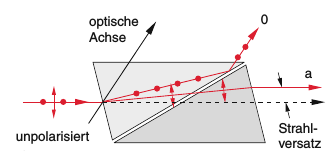
\includegraphics{nicol}
			\caption{Strahlengang im Nicol'schen Prisma}
			\label{fig:Abb7}
		\end{figure}
		Ein negativ einachsiger ($n_o>n_e$) Kristall wird schräg zur optischen Achse durchgeschnitten und mit einem durchsichtigen Kleber wieder zusammengeklebt, sodass $n_o>n_K>n_e$ erfüllt ist. Aufgrund der unterschiedlichen Einfallswinkel der Strahlen auf die Kristall-Kleber-Grenzfläche kann so bewirkt werden, dass der Einfallswinkel des ordentlichen Strahls größer ist, als der Totalreflexionswinkel. Es tritt daher nur der außerordentliche Strahl aus, der parallel zur Einfallsebene und somit linear polarisiert ist.
	\item Was versteht man unter Spannungsdoppelbrechung?
		\subitem Unter Spannungsdoppelbrechung versteht man die Eigenschaft von Materialen, unter mechanischer Zugspannung Doppelbrechung aufzuweisen, also in verschiedenen Richtungen verschiedene Brechungsindizes zu besitzen.
	\item Wie kann man Licht eines bestimmten Polarisationstyps erzeugen und nachweisen?
		\subitem Die Erzeugung linear polarisierten Lichts aus unpolarisiertem geschieht zum Beispiel durch bereits beschriebene Mechanismen der Doppelbrechung. Daraus lässt sich mittels eines $\lambda/4-$Plättchens zirkular polarisiertes Licht erzeugen. Der Nachweis dieser Polarisationen geschieht durch Linearpolarisatoren im ersten Fall bzw. durch die Kombination eines $\lambda/4-$Plättchens und eines Linearpolarisators im zweiten Fall.
\end{enumerate}
\section{Durchführung}
\subsection{Doppelbrechung}
Legen Sie den Kalkspat-Kristall auf Millimeterpapier, auf das Sie zuvor ein farbiges Kreuz gezeichnet haben. Bestimmen Sie nun durch Drehen des Kristalls die Strahlverschiebung $s$. Fällt das Licht senkrecht auf die Oberfläche des Kristalls, so kann aus der Stahlverschiebung und der Kristalldicke $d$ der Ablenkwinkel berechnet werden (siehe Abb.  \ref{fig:Abb8}).
\begin{figure}[!h]
	\centering
	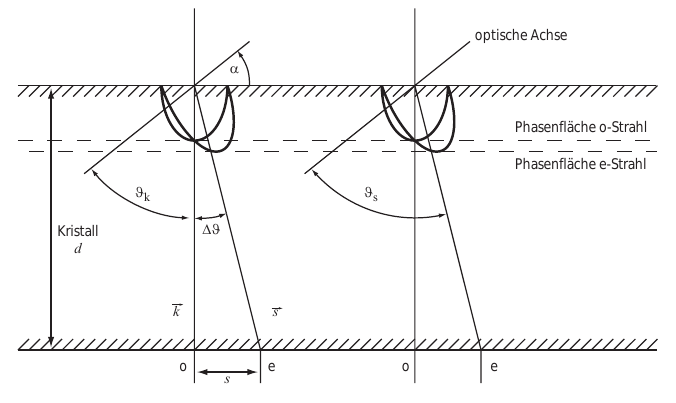
\includegraphics{doppelbrechung}
	\caption{Ordentlicher und außerordentlicher Strahl im Kalkspat}
	\label{fig:Abb8}
\end{figure} 
Die Formel zur Berechnung des Ablenkwinkels $\Delta\vartheta$ können Sie der Abb. \ref{fig:Abb8} entnehmen. Vergleichen Sie die gemessene Strahlverschiebung $s$ mit dem theoretischen Wert der Strahlverschiebung des Kalkspats. Die Winkel $\vartheta_k$ und $\vartheta_s$ sind wie folgt verknüpft:
\begin{equation}
	\label{eq:7}\frac{\tan\vartheta_s}{\tan\vartheta_k}=\frac{n_o^2}{n_e^2}
\end{equation}
Die optische Achse tritt unter dem Winkel $\alpha=\SI{45.49}{\degree}$ aus der Kristalloberfläche aus. Setzen Sie $\vartheta_s$ aus Gleichung \eqref{eq:7} in ihre Gleichung für die Strahlverschiebung ein. Mit $\vartheta_k=\SI{90}{\degree}-\alpha$ können Sie den theoretischen Wert der Strahlverschiebung berechnen.
\subsection{Gesetz von Malus}\label{GvM}
Machen Sie sich zunächst mit dem Polarisator vertraut. Überprüfen Sie die Angabe der Durchlassrichtung (E-Vektor). Beobachten Sie die Polarisationseigenschaften von Gegenständen in ihrer Umgebung sowie der Atmosphäre und der Wolken und notieren Sie diese. Wie schwingt der E-Vektor des beobachteten Lichtes?

Für die Messungen stellen Sie einen Polarisator und einen Analysator mit Winkelmessvorrichtung in den Strahlengang (vgl Abb. pl.2). Machen Sie sich zunächst klar, wann deren Durchlassrichtungen parallel bzw. senkrecht zueinander stehen. Messen Sie nun die Winkelintensitätsverteilung von polarisiertem Licht, wobei Sie den Winkel zwischen Polarisator und Analysator kontinuierlich ändern. Überprüfen Sie das Gesetz von Malus durch eine geeignete graphische Darstellung ihrer Messwerte. Tragen Sie dann ihre Messwerte in Polarkoordinatenpapier ein. Was sagt die Graphik aus?
\subsection{$\lambda/4-$Plättchen}\label{4tel}
Stellen Sie nun ein $\lambda/4-$Plättchen zwischen den Polarisator und den Analysator in den Strahlengang. Orientieren Sie das Plättchen mit Hilfe der Polarisatoren. Erzeugen Sie nun elliptisch polarisiertes Licht. Überlegen Sie sich wie das $\lambda/4-$Plättchen eingestellt werden muss! Messen Sie die Intensitätsverteilung wie unter \ref{GvM} und tragen Sie ihre Messwerte in Polarkoordinatenpapier ein. Stellen Sie das $\lambda/4-$Plättchen nun so in den Strahlengang, dass es zirkular polarisiertes Licht erzeugt. Messen Sie erneut die Intensitätsverteilung wie unter \ref{GvM} und tragen Sie ihre Messwerte in Polarkoordinatenpapier ein.
\subsection{$\lambda/2-$Plättchen}\label{halb}
Tauschen Sie das $\lambda/4-$Plättchen durch ein $\lambda/2-$Plättchen aus und orientieren Sie dieses im Strahlengang. Drehen Sie es anschließend um $\SI{20}{\degree}$ zur eingestellten Vorzugsrichtung. Messen Sie die Intensitätsverteilung und tragen Sie Ihre Messwerte in Polarkoordinatenpapier ein. Was schließen Sie aus dem Ergebnis?
\subsection{selbstgebaut...}
Wiederholen Sie die Aufgaben \ref{4tel} und \ref{halb} mit "`selbstgebauten"' Plättchen.
\subsection{Beobachtungen}
Betrachten Sie transparente Medien unter gekreuzten Polarisatoren und schreiben Sie Ihre Beobachtungen nieder.